\chapter{Einleitung}
\vspace{-1.2cm}
Im folgenden Kapitel wird die Grundlage für die vorliegende Bachelorarbeit geschaffen. Hierbei werden die Motivation und das Ziel der Arbeit erläutert, um einen klaren Überblick über den Themenkontext zu bieten. Desweiteren werden die Anforderungen an das System gestellt.

\section{Pepperl + Fuchs / HMI}\label{sec:PFHMI}
Die \ac{p+f} wurde 1945 von Walter Pepperl und Ludwig Fuchs gegründet. Anfangs war sie eine Radioreperaturwekstadt, welche sich erst nach der Entwicklung eines eigenen Näherungsschalters so wie eines eigensicheren Transistorverstärkers auf das gebiet der Elektronik ausweitete. Inzwischen entwickelt, produziert und vertreibt \ac{p+f} Baugruppen und Sensoren für den Automatisierungsmarkt.\\
\vspace{-1cm}
\begin{flushleft}
    \begin{figure}[h!]
        \centering
        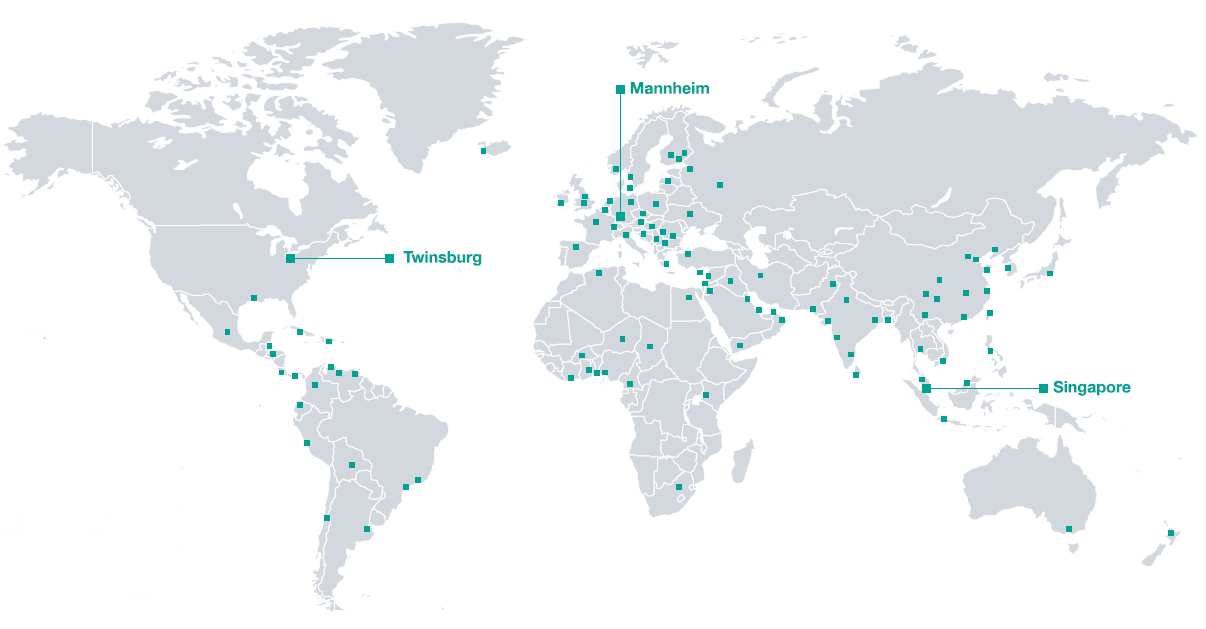
\includegraphics[width=1\linewidth]{P+F_Standorte.png}
        \caption{Standorte der Pepperl+Fuchs SE}
        \label{fig:StandortePF}
    \end{figure}
\end{flushleft}
Im Bereich der Prozessautomation ist \ac*{p+f} führender Hersteller industrieller Sicherheitsausstattungen. Das Produktportfolio umfasst eine Reihe von industrieller Computer Systeme, welche zur Überwachung und Steuerung von Prozessen in Explosionsgefährdeten Bereichen genutzt werde. Die \ac{hmi} Abteilung beschäftigt sich mit der Entwicklung diser Systeme, welche eine Schnitstelle zwischen Mensch und Maschiene bilden. Da es eine vielzahl an Anwendungen für \ac{hmi} Systeme im Explosionsgefährdeten bereichen gibt, wurde die Produktfamilie \textit{VisuNet} speziell für den Einsatz in diesen Zohnen Konzipiert. Solche Ex-Zohnen sind überall da zu finden, wo Explosionsgefährliche stoffe gelagert oder gehandhabt werden. In diesen Zohnen kann durch Gas oder Staub, eine explosionsfähige Atmosphäre entstehen. Zudem kommen auch Umwelttechnische Einflüsse wie Sonne, Nässe, Hitze und Kälte, aber auch Einflüsse welche beispielsweise durch die Reinigung mit aggresiven Chemikalien entstehen, hinzu. Um in einer solchen Computerfeindlichen Umgebung dennoch ein Prozessleitsystem zu Integrieren, setzte \ac{p+f} mit den \textit{VisuNet} Remote Monitoren auf die Thin-Client-Technologie. Hierbei verbindet sich der Ex-Geschützte Monitor aus der Explosionsgefährdeten Zohne mit der Zentralen, meist Leistungsstärkeren, Recheneinheit in der No-Ex-Zohne. Eingaben über Tastatur und Maus werden anschließend über den Monitor an die Zentrale Recheneinheit weitergeleitet, welche anschließend die neuen ausgaben an den Monitor zurückschickt.  

\section{Intention und Ziel der Arbeit}\label{sec:IZA}
Durch die Ex-Schutz Zertifizierung der \textit{VisuNet} Platformen, sind Vorgeschriebene Betriebstemperaturgrenzen der Systeme einzuhalten. Durch integrierte Schutzschaltungen und weitere Sicherheitsmechanismen ist es den Geräten nicht möglich diese Grenzwerte zu überschreiten. Durch den Einsatz dieser Geräte in Industriellen Umgebungen, können sich verschiedene Umwelteinflüsse wie beispielsweise die Sonneneinstrahlung, negativ auf das System auswirken. Zudem können diese Umwelteinflüsse das gerät auch in Systemzustände bringen, welche den Zertifizierungsrichtlinien wiedersprechen. Durch eine Falsche einschätzung der Umweltfaktoren werden solche unzulässigen bzw schädlichen Betriebe vom Endkunden meist nicht wargenommen.\\
Eine Möglichkeit dem zu Begegnen, ist die auf  der Hardware verbaute Sensorik zu nutzen, um den Zustand des Systems zu überwachen. Aus den Daten können anschließend Rückschlusse, auf Nutzungsverhalten und die daraus resultierenden Betriebszustände gezogen wereden. Dem Nutzer können somit wichtige Informationen zum Systemzustand vermittelt werden, sodas Schädliche bzw. Kritische zustände endekt und vermieden werden können.\\
Primäres Ziel dieser Bachelorarbeit ist daher, die prototypische Entwicklung einer Hardware-Health Monitoring Lösung für die \acl{p+f} \ac{hmi} Plattformen \textit{VisuNet GXP} und \textit{FLX}. Hierbei soll eine Architektur und Konzepterweiterung für den Aufbau einer verteilten Health-Monitoring Lösung, welche möglichst plattformunabhängig ausgeführt werden kann, erstellt werden. Dazu gilt es Sensoren und Messwerte, welche bei der„Health“- Status Definition berücksichtigt werden sollen, auszuwählen und auszulesen. Des Weiteren soll ein Modell definiert werden, welches die Sensor-Messerte in einen plattformspezifischen Health-Status übersetzt um dem Benutzer den aktuellen Zustand (Ampel-Prinzip) mitzuteilen. Als prototypische Umsetzung soll ein Health Agent, entwickelt werden, welche Geräte-Daten (z.B. aktuelle Temperatur) der \ac{hmi} Systeme ausliest, abspeichert, in der VisuNet RM Shell 6 dem Benutzer visualisiert und per Netzwerkprotokoll (z.B. MQTT oder SNMP) auch einen zentralen Servern bereitstellen kann.    

\section{Anforderungen}
Durch das in Abschnitt \ref{sec:IZA} erläuterte Ziel dieser Arbeit, ergeben sich die unten Aufgelisteten Anforderungen.
\begin{enumerate}
    \item Schnitestelle zur Datenerfassung
    \begin{enumerate}
        \item Aulesen der System Sensorik\\
        Das System benötigt eine zentrale Schnitstelle, welche das Auslesen der Sensoren der VisuNet Platformen ermölgicht. Die \textit{VisuNet} Platformen unterscheiden sich in der ausgestatteten Elektronik so weit, das verschiedene Ansätze zum Auswerten dieser Benötigt werden. 
        \item Speichern der Ausgelesenen Messwerte\\
        Zur verwaltung der gesammelten Daten, benötigt das System eine Zentrale Datenbank. Diese muss über eine übersichtliche und Effiziente struktur verfügen, welche das Verarbeiten der gesammelten Daten im Nachgang ermöglicht.
    \end{enumerate}
    
    \item Datenverarbeitung
    \begin{enumerate}
        \item Ermittelung des Health Status\\
        Für die jeweiligen \textit{VisuNet} Platformen soll der System Helth Satus ermittelt werden. Dieser Soll eine aussage über den Betrieb des Systems geben. 
        \item Ermittelung der Health Status Historie\\
        Über die gesammelten Health Status Daten soll zudem eine Historie erstellt werden. Diese soll eine Aussage über das generelle Nutzungsverhalten des Systems treffen. 
        \item Ermittelung der System Reliability\\
        Zudem soll eine aussage über den zustand des Systems, mittels Reliability, getroffen werden. 
    \end{enumerate}

    \item Datendistribution
    \begin{enumerate}
        \item Visualisierung der Systemdaten\\
        Die gesammelten Daten des Systems sollen über ein Dashboard visualisiert werden. In diesem soll dem Kunden, eine Auswertung des Systemverhaltens präsentiert werden. 
        \item Distribution der Daten zu einem externen Service\\
        Die gesammelten Daten des Systems sollen über ein Netzwerkprotokoll (MQTT, SNMP) an einen Dritten Service übermittelt werden können.
    \end{enumerate}

   \end{enumerate}

